% Options for packages loaded elsewhere
\PassOptionsToPackage{unicode}{hyperref}
\PassOptionsToPackage{hyphens}{url}
%
\documentclass[
]{article}
\title{Assignment 5: Data Visualization}
\author{Shana Shapiro Section \#1}
\date{}

\usepackage{amsmath,amssymb}
\usepackage{lmodern}
\usepackage{iftex}
\ifPDFTeX
  \usepackage[T1]{fontenc}
  \usepackage[utf8]{inputenc}
  \usepackage{textcomp} % provide euro and other symbols
\else % if luatex or xetex
  \usepackage{unicode-math}
  \defaultfontfeatures{Scale=MatchLowercase}
  \defaultfontfeatures[\rmfamily]{Ligatures=TeX,Scale=1}
\fi
% Use upquote if available, for straight quotes in verbatim environments
\IfFileExists{upquote.sty}{\usepackage{upquote}}{}
\IfFileExists{microtype.sty}{% use microtype if available
  \usepackage[]{microtype}
  \UseMicrotypeSet[protrusion]{basicmath} % disable protrusion for tt fonts
}{}
\makeatletter
\@ifundefined{KOMAClassName}{% if non-KOMA class
  \IfFileExists{parskip.sty}{%
    \usepackage{parskip}
  }{% else
    \setlength{\parindent}{0pt}
    \setlength{\parskip}{6pt plus 2pt minus 1pt}}
}{% if KOMA class
  \KOMAoptions{parskip=half}}
\makeatother
\usepackage{xcolor}
\IfFileExists{xurl.sty}{\usepackage{xurl}}{} % add URL line breaks if available
\IfFileExists{bookmark.sty}{\usepackage{bookmark}}{\usepackage{hyperref}}
\hypersetup{
  pdftitle={Assignment 5: Data Visualization},
  pdfauthor={Shana Shapiro Section \#1},
  hidelinks,
  pdfcreator={LaTeX via pandoc}}
\urlstyle{same} % disable monospaced font for URLs
\usepackage[margin=2.54cm]{geometry}
\usepackage{color}
\usepackage{fancyvrb}
\newcommand{\VerbBar}{|}
\newcommand{\VERB}{\Verb[commandchars=\\\{\}]}
\DefineVerbatimEnvironment{Highlighting}{Verbatim}{commandchars=\\\{\}}
% Add ',fontsize=\small' for more characters per line
\usepackage{framed}
\definecolor{shadecolor}{RGB}{248,248,248}
\newenvironment{Shaded}{\begin{snugshade}}{\end{snugshade}}
\newcommand{\AlertTok}[1]{\textcolor[rgb]{0.94,0.16,0.16}{#1}}
\newcommand{\AnnotationTok}[1]{\textcolor[rgb]{0.56,0.35,0.01}{\textbf{\textit{#1}}}}
\newcommand{\AttributeTok}[1]{\textcolor[rgb]{0.77,0.63,0.00}{#1}}
\newcommand{\BaseNTok}[1]{\textcolor[rgb]{0.00,0.00,0.81}{#1}}
\newcommand{\BuiltInTok}[1]{#1}
\newcommand{\CharTok}[1]{\textcolor[rgb]{0.31,0.60,0.02}{#1}}
\newcommand{\CommentTok}[1]{\textcolor[rgb]{0.56,0.35,0.01}{\textit{#1}}}
\newcommand{\CommentVarTok}[1]{\textcolor[rgb]{0.56,0.35,0.01}{\textbf{\textit{#1}}}}
\newcommand{\ConstantTok}[1]{\textcolor[rgb]{0.00,0.00,0.00}{#1}}
\newcommand{\ControlFlowTok}[1]{\textcolor[rgb]{0.13,0.29,0.53}{\textbf{#1}}}
\newcommand{\DataTypeTok}[1]{\textcolor[rgb]{0.13,0.29,0.53}{#1}}
\newcommand{\DecValTok}[1]{\textcolor[rgb]{0.00,0.00,0.81}{#1}}
\newcommand{\DocumentationTok}[1]{\textcolor[rgb]{0.56,0.35,0.01}{\textbf{\textit{#1}}}}
\newcommand{\ErrorTok}[1]{\textcolor[rgb]{0.64,0.00,0.00}{\textbf{#1}}}
\newcommand{\ExtensionTok}[1]{#1}
\newcommand{\FloatTok}[1]{\textcolor[rgb]{0.00,0.00,0.81}{#1}}
\newcommand{\FunctionTok}[1]{\textcolor[rgb]{0.00,0.00,0.00}{#1}}
\newcommand{\ImportTok}[1]{#1}
\newcommand{\InformationTok}[1]{\textcolor[rgb]{0.56,0.35,0.01}{\textbf{\textit{#1}}}}
\newcommand{\KeywordTok}[1]{\textcolor[rgb]{0.13,0.29,0.53}{\textbf{#1}}}
\newcommand{\NormalTok}[1]{#1}
\newcommand{\OperatorTok}[1]{\textcolor[rgb]{0.81,0.36,0.00}{\textbf{#1}}}
\newcommand{\OtherTok}[1]{\textcolor[rgb]{0.56,0.35,0.01}{#1}}
\newcommand{\PreprocessorTok}[1]{\textcolor[rgb]{0.56,0.35,0.01}{\textit{#1}}}
\newcommand{\RegionMarkerTok}[1]{#1}
\newcommand{\SpecialCharTok}[1]{\textcolor[rgb]{0.00,0.00,0.00}{#1}}
\newcommand{\SpecialStringTok}[1]{\textcolor[rgb]{0.31,0.60,0.02}{#1}}
\newcommand{\StringTok}[1]{\textcolor[rgb]{0.31,0.60,0.02}{#1}}
\newcommand{\VariableTok}[1]{\textcolor[rgb]{0.00,0.00,0.00}{#1}}
\newcommand{\VerbatimStringTok}[1]{\textcolor[rgb]{0.31,0.60,0.02}{#1}}
\newcommand{\WarningTok}[1]{\textcolor[rgb]{0.56,0.35,0.01}{\textbf{\textit{#1}}}}
\usepackage{graphicx}
\makeatletter
\def\maxwidth{\ifdim\Gin@nat@width>\linewidth\linewidth\else\Gin@nat@width\fi}
\def\maxheight{\ifdim\Gin@nat@height>\textheight\textheight\else\Gin@nat@height\fi}
\makeatother
% Scale images if necessary, so that they will not overflow the page
% margins by default, and it is still possible to overwrite the defaults
% using explicit options in \includegraphics[width, height, ...]{}
\setkeys{Gin}{width=\maxwidth,height=\maxheight,keepaspectratio}
% Set default figure placement to htbp
\makeatletter
\def\fps@figure{htbp}
\makeatother
\setlength{\emergencystretch}{3em} % prevent overfull lines
\providecommand{\tightlist}{%
  \setlength{\itemsep}{0pt}\setlength{\parskip}{0pt}}
\setcounter{secnumdepth}{-\maxdimen} % remove section numbering
\ifLuaTeX
  \usepackage{selnolig}  % disable illegal ligatures
\fi

\begin{document}
\maketitle

\hypertarget{overview}{%
\subsection{OVERVIEW}\label{overview}}

This exercise accompanies the lessons in Environmental Data Analytics on
Data Visualization

\hypertarget{directions}{%
\subsection{Directions}\label{directions}}

\begin{enumerate}
\def\labelenumi{\arabic{enumi}.}
\tightlist
\item
  Change ``Student Name'' on line 3 (above) with your name.
\item
  Work through the steps, \textbf{creating code and output} that fulfill
  each instruction.
\item
  Be sure to \textbf{answer the questions} in this assignment document.
\item
  When you have completed the assignment, \textbf{Knit} the text and
  code into a single PDF file.
\item
  After Knitting, submit the completed exercise (PDF file) to the
  dropbox in Sakai. Add your last name into the file name (e.g.,
  ``Fay\_A05\_DataVisualization.Rmd'') prior to submission.
\end{enumerate}

The completed exercise is due on Monday, February 14 at 7:00 pm.

\hypertarget{set-up-your-session}{%
\subsection{Set up your session}\label{set-up-your-session}}

\begin{enumerate}
\def\labelenumi{\arabic{enumi}.}
\item
  Set up your session. Verify your working directory and load the
  tidyverse and cowplot packages. Upload the NTL-LTER processed data
  files for nutrients and chemistry/physics for Peter and Paul Lakes
  (use the tidy
  {[}\texttt{NTL-LTER\_Lake\_Chemistry\_Nutrients\_PeterPaul\_Processed.csv}{]}
  version) and the processed data file for the Niwot Ridge litter
  dataset (use the
  {[}\texttt{NEON\_NIWO\_Litter\_mass\_trap\_Processed.csv}{]} version).
\item
  Make sure R is reading dates as date format; if not change the format
  to date.
\end{enumerate}

\begin{Shaded}
\begin{Highlighting}[]
\CommentTok{\#1 }
\FunctionTok{getwd}\NormalTok{()}
\end{Highlighting}
\end{Shaded}

\begin{verbatim}
## [1] "Z:/EnvironmentalDataAnalytics/Environmental_Data_Analytics_2022/Assignments"
\end{verbatim}

\begin{Shaded}
\begin{Highlighting}[]
\FunctionTok{library}\NormalTok{(}\StringTok{"tidyverse"}\NormalTok{,}\StringTok{"ggplot2"}\NormalTok{)}
\end{Highlighting}
\end{Shaded}

\begin{verbatim}
## Warning: package 'tidyverse' was built under R version 4.0.5
\end{verbatim}

\begin{verbatim}
## -- Attaching packages --------------------------------------- tidyverse 1.3.1 --
\end{verbatim}

\begin{verbatim}
## v ggplot2 3.3.5     v purrr   0.3.4
## v tibble  3.1.6     v dplyr   1.0.7
## v tidyr   1.1.4     v stringr 1.4.0
## v readr   2.1.1     v forcats 0.5.1
\end{verbatim}

\begin{verbatim}
## Warning: package 'ggplot2' was built under R version 4.0.5
\end{verbatim}

\begin{verbatim}
## Warning: package 'tibble' was built under R version 4.0.5
\end{verbatim}

\begin{verbatim}
## Warning: package 'tidyr' was built under R version 4.0.5
\end{verbatim}

\begin{verbatim}
## Warning: package 'readr' was built under R version 4.0.5
\end{verbatim}

\begin{verbatim}
## Warning: package 'purrr' was built under R version 4.0.5
\end{verbatim}

\begin{verbatim}
## Warning: package 'dplyr' was built under R version 4.0.5
\end{verbatim}

\begin{verbatim}
## Warning: package 'stringr' was built under R version 4.0.5
\end{verbatim}

\begin{verbatim}
## Warning: package 'forcats' was built under R version 4.0.5
\end{verbatim}

\begin{verbatim}
## -- Conflicts ------------------------------------------ tidyverse_conflicts() --
## x dplyr::filter() masks stats::filter()
## x dplyr::lag()    masks stats::lag()
\end{verbatim}

\begin{Shaded}
\begin{Highlighting}[]
\FunctionTok{library}\NormalTok{(}\StringTok{"cowplot"}\NormalTok{)}
\end{Highlighting}
\end{Shaded}

\begin{verbatim}
## Warning: package 'cowplot' was built under R version 4.0.5
\end{verbatim}

\begin{Shaded}
\begin{Highlighting}[]
\NormalTok{lakes }\OtherTok{\textless{}{-}} \FunctionTok{read.csv}\NormalTok{(}\StringTok{"../Data/Processed/NTL{-}LTER\_Lake\_Chemistry\_Nutrients\_PeterPaul\_Processed.csv"}\NormalTok{)}
\NormalTok{litter }\OtherTok{\textless{}{-}} \FunctionTok{read.csv}\NormalTok{(}\StringTok{"../Data/Processed/NEON\_NIWO\_Litter\_mass\_trap\_Processed.csv"}\NormalTok{)}

\CommentTok{\#2}
\FunctionTok{class}\NormalTok{(lakes}\SpecialCharTok{$}\NormalTok{sampledate) }\CommentTok{\#character}
\end{Highlighting}
\end{Shaded}

\begin{verbatim}
## [1] "character"
\end{verbatim}

\begin{Shaded}
\begin{Highlighting}[]
\NormalTok{lakes}\SpecialCharTok{$}\NormalTok{sampledate }\OtherTok{\textless{}{-}} \FunctionTok{as.Date}\NormalTok{(lakes}\SpecialCharTok{$}\NormalTok{sampledate)}
\FunctionTok{class}\NormalTok{(lakes}\SpecialCharTok{$}\NormalTok{sampledate) }\CommentTok{\#date }
\end{Highlighting}
\end{Shaded}

\begin{verbatim}
## [1] "Date"
\end{verbatim}

\begin{Shaded}
\begin{Highlighting}[]
\FunctionTok{class}\NormalTok{(litter}\SpecialCharTok{$}\NormalTok{collectDate) }\CommentTok{\#character }
\end{Highlighting}
\end{Shaded}

\begin{verbatim}
## [1] "character"
\end{verbatim}

\begin{Shaded}
\begin{Highlighting}[]
\NormalTok{litter}\SpecialCharTok{$}\NormalTok{collectDate }\OtherTok{\textless{}{-}} \FunctionTok{as.Date}\NormalTok{(litter}\SpecialCharTok{$}\NormalTok{collectDate)}
\FunctionTok{class}\NormalTok{(litter}\SpecialCharTok{$}\NormalTok{collectDate) }\CommentTok{\#date }
\end{Highlighting}
\end{Shaded}

\begin{verbatim}
## [1] "Date"
\end{verbatim}

\hypertarget{define-your-theme}{%
\subsection{Define your theme}\label{define-your-theme}}

\begin{enumerate}
\def\labelenumi{\arabic{enumi}.}
\setcounter{enumi}{2}
\tightlist
\item
  Build a theme and set it as your default theme.
\end{enumerate}

\begin{Shaded}
\begin{Highlighting}[]
\CommentTok{\#3}
\NormalTok{mytheme }\OtherTok{\textless{}{-}} \FunctionTok{theme\_classic}\NormalTok{(}\AttributeTok{base\_size =} \DecValTok{14}\NormalTok{) }\SpecialCharTok{+}
  \FunctionTok{theme}\NormalTok{(}\AttributeTok{axis.text =} \FunctionTok{element\_text}\NormalTok{(}\AttributeTok{color =} \StringTok{"black"}\NormalTok{), }
        \AttributeTok{legend.position =} \StringTok{"right"}\NormalTok{,}
        \AttributeTok{plot.title =} \FunctionTok{element\_text}\NormalTok{(}\AttributeTok{face =} \StringTok{"bold"}\NormalTok{,}\AttributeTok{size=}\DecValTok{12}\NormalTok{),}
        \AttributeTok{axis.ticks =} \FunctionTok{element\_line}\NormalTok{(}\AttributeTok{colour=}\StringTok{"grey70"}\NormalTok{, }\AttributeTok{size =} \FloatTok{0.2}\NormalTok{),}
        \AttributeTok{panel.grid.major =} \FunctionTok{element\_line}\NormalTok{(}\AttributeTok{colour=}\StringTok{"grey70"}\NormalTok{, }\AttributeTok{size =} \FloatTok{0.2}\NormalTok{),}
        \AttributeTok{panel.grid.minor =} \FunctionTok{element\_blank}\NormalTok{())}
\end{Highlighting}
\end{Shaded}

\hypertarget{create-graphs}{%
\subsection{Create graphs}\label{create-graphs}}

For numbers 4-7, create ggplot graphs and adjust aesthetics to follow
best practices for data visualization. Ensure your theme, color
palettes, axes, and additional aesthetics are edited accordingly.

\begin{enumerate}
\def\labelenumi{\arabic{enumi}.}
\setcounter{enumi}{3}
\tightlist
\item
  {[}NTL-LTER{]} Plot total phosphorus (\texttt{tp\_ug}) by phosphate
  (\texttt{po4}), with separate aesthetics for Peter and Paul lakes. Add
  a line of best fit and color it black. Adjust your axes to hide
  extreme values (hint: change the limits using \texttt{xlim()} and
  \texttt{ylim()}).
\end{enumerate}

\begin{Shaded}
\begin{Highlighting}[]
\CommentTok{\#4}
\NormalTok{phos }\OtherTok{\textless{}{-}} \FunctionTok{ggplot}\NormalTok{(lakes, }\FunctionTok{aes}\NormalTok{(}\AttributeTok{x=}\NormalTok{tp\_ug, }\AttributeTok{y=}\NormalTok{po4, }\AttributeTok{color =}\NormalTok{ lakename)) }\SpecialCharTok{+} 
  \FunctionTok{geom\_point}\NormalTok{() }\SpecialCharTok{+}
\NormalTok{  mytheme }\SpecialCharTok{+}
  \FunctionTok{xlim}\NormalTok{(}\DecValTok{0}\NormalTok{,}\DecValTok{150}\NormalTok{) }\SpecialCharTok{+} 
  \FunctionTok{ylim}\NormalTok{(}\DecValTok{0}\NormalTok{,}\DecValTok{50}\NormalTok{) }\SpecialCharTok{+}
  \FunctionTok{geom\_smooth}\NormalTok{(}\FunctionTok{aes}\NormalTok{(}\AttributeTok{group=}\NormalTok{lakename), }\AttributeTok{method=}\StringTok{"lm"}\NormalTok{, }\AttributeTok{color =} \StringTok{"black"}\NormalTok{, }\AttributeTok{size=}\FloatTok{0.5}\NormalTok{) }\SpecialCharTok{+}
  \FunctionTok{ylab}\NormalTok{(}\FunctionTok{expression}\NormalTok{(}\StringTok{"PO"}\NormalTok{[}\DecValTok{4}\NormalTok{]))}
\FunctionTok{print}\NormalTok{(phos)}
\end{Highlighting}
\end{Shaded}

\begin{verbatim}
## `geom_smooth()` using formula 'y ~ x'
\end{verbatim}

\begin{verbatim}
## Warning: Removed 21948 rows containing non-finite values (stat_smooth).
\end{verbatim}

\begin{verbatim}
## Warning: Removed 21948 rows containing missing values (geom_point).
\end{verbatim}

\begin{verbatim}
## Warning: Removed 2 rows containing missing values (geom_smooth).
\end{verbatim}

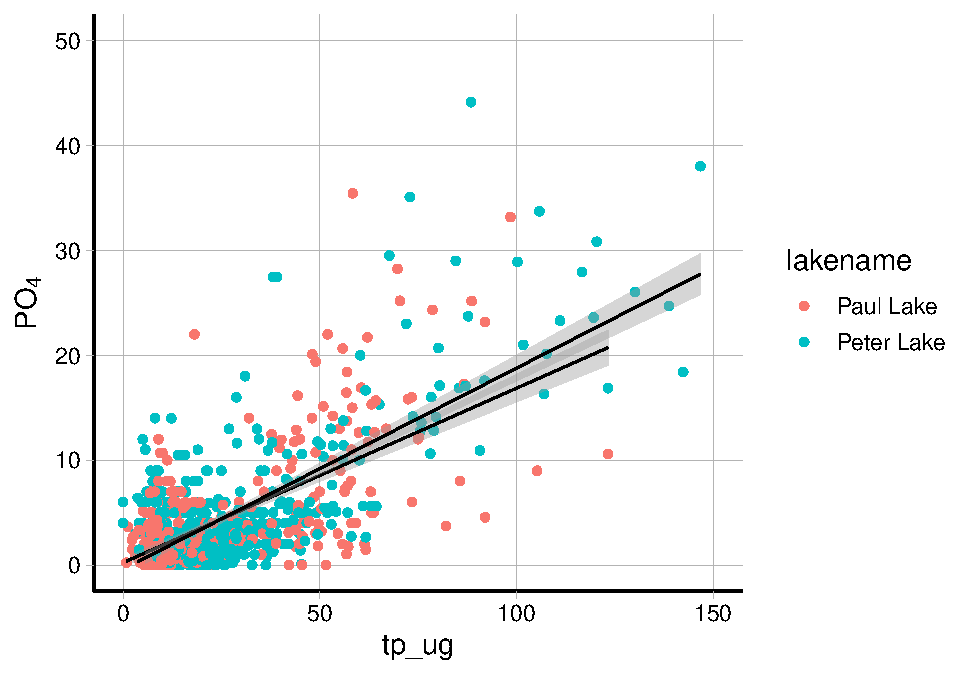
\includegraphics{A05_DataVisualization_files/figure-latex/unnamed-chunk-3-1.pdf}

\begin{enumerate}
\def\labelenumi{\arabic{enumi}.}
\setcounter{enumi}{4}
\tightlist
\item
  {[}NTL-LTER{]} Make three separate boxplots of (a) temperature, (b)
  TP, and (c) TN, with month as the x axis and lake as a color
  aesthetic. Then, create a cowplot that combines the three graphs. Make
  sure that only one legend is present and that graph axes are aligned.
\end{enumerate}

\begin{Shaded}
\begin{Highlighting}[]
\CommentTok{\#5}
\NormalTok{temp }\OtherTok{\textless{}{-}} \FunctionTok{ggplot}\NormalTok{(lakes, }\FunctionTok{aes}\NormalTok{(}\AttributeTok{x=}\FunctionTok{as.factor}\NormalTok{(month), }\AttributeTok{y=}\NormalTok{temperature\_C, }\AttributeTok{color =}\NormalTok{ lakename)) }\SpecialCharTok{+} 
  \FunctionTok{geom\_boxplot}\NormalTok{() }\SpecialCharTok{+} 
  \FunctionTok{ylab}\NormalTok{(}\FunctionTok{expression}\NormalTok{(}\StringTok{"Temperature C"}\NormalTok{)) }\SpecialCharTok{+}
  \FunctionTok{xlab}\NormalTok{(}\FunctionTok{expression}\NormalTok{(}\StringTok{"Month"}\NormalTok{)) }\SpecialCharTok{+} 
\NormalTok{  mytheme}
\FunctionTok{print}\NormalTok{(temp)}
\end{Highlighting}
\end{Shaded}

\begin{verbatim}
## Warning: Removed 3566 rows containing non-finite values (stat_boxplot).
\end{verbatim}

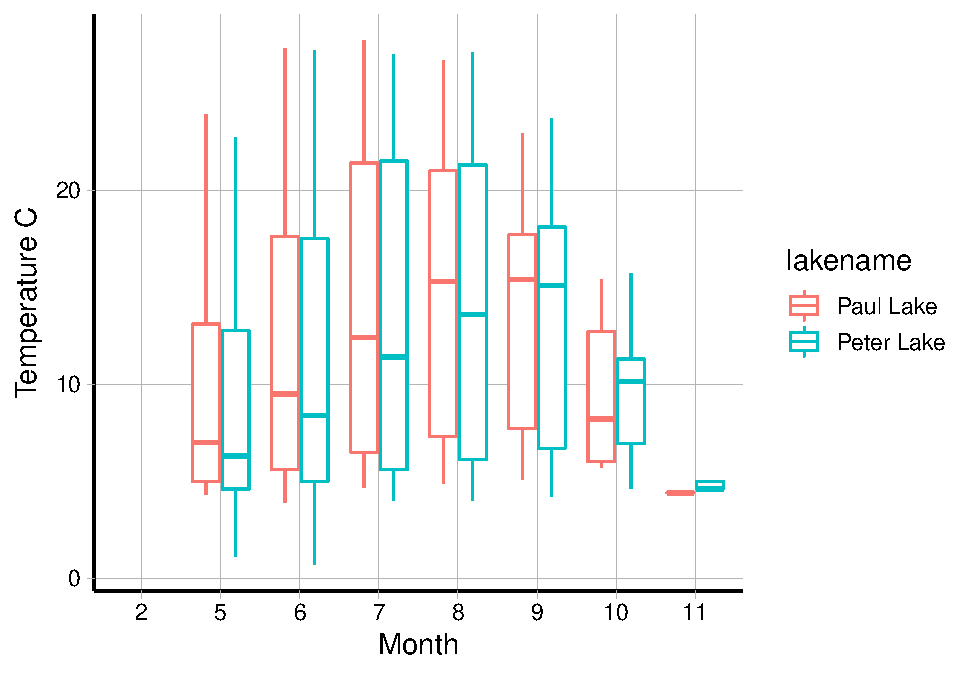
\includegraphics{A05_DataVisualization_files/figure-latex/unnamed-chunk-4-1.pdf}

\begin{Shaded}
\begin{Highlighting}[]
\NormalTok{TP }\OtherTok{\textless{}{-}} \FunctionTok{ggplot}\NormalTok{(lakes, }\FunctionTok{aes}\NormalTok{(}\AttributeTok{x=}\FunctionTok{as.factor}\NormalTok{(month),}\AttributeTok{y=}\NormalTok{tp\_ug,}\AttributeTok{color=}\NormalTok{lakename)) }\SpecialCharTok{+} 
  \FunctionTok{geom\_boxplot}\NormalTok{() }\SpecialCharTok{+} 
  \FunctionTok{ylab}\NormalTok{(}\FunctionTok{expression}\NormalTok{(}\StringTok{"TP"}\NormalTok{)) }\SpecialCharTok{+}
  \FunctionTok{xlab}\NormalTok{(}\FunctionTok{expression}\NormalTok{(}\StringTok{"Month"}\NormalTok{)) }\SpecialCharTok{+} 
\NormalTok{  mytheme }
\FunctionTok{print}\NormalTok{(TP)}
\end{Highlighting}
\end{Shaded}

\begin{verbatim}
## Warning: Removed 20729 rows containing non-finite values (stat_boxplot).
\end{verbatim}

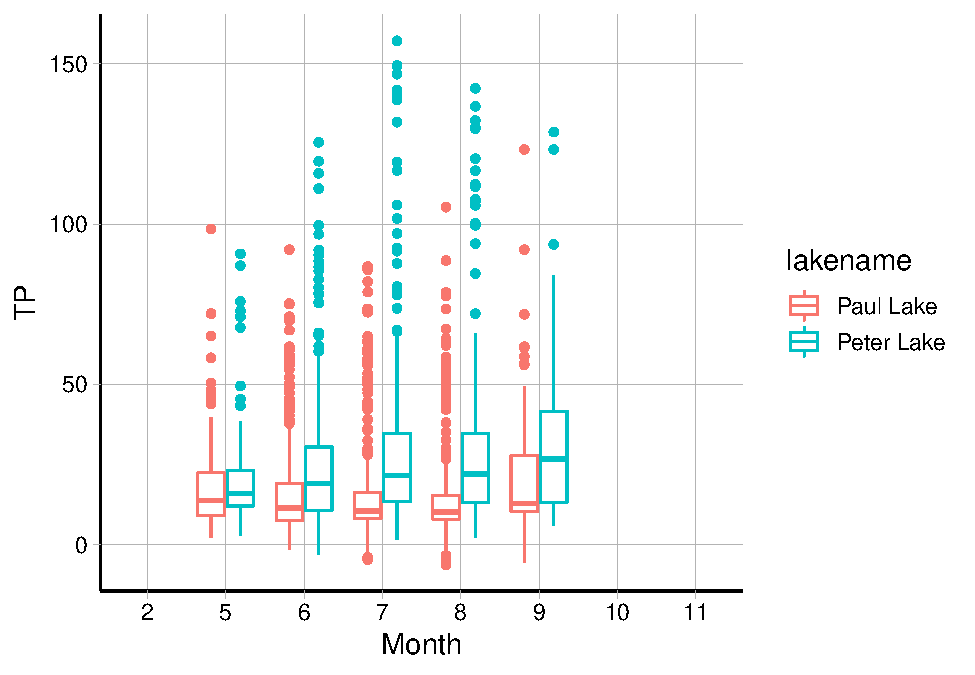
\includegraphics{A05_DataVisualization_files/figure-latex/unnamed-chunk-4-2.pdf}

\begin{Shaded}
\begin{Highlighting}[]
\NormalTok{TN }\OtherTok{\textless{}{-}} \FunctionTok{ggplot}\NormalTok{(lakes, }\FunctionTok{aes}\NormalTok{(}\AttributeTok{x=}\FunctionTok{as.factor}\NormalTok{(month),}\AttributeTok{y=}\NormalTok{tn\_ug,}\AttributeTok{color=}\NormalTok{lakename))}\SpecialCharTok{+}
  \FunctionTok{geom\_boxplot}\NormalTok{() }\SpecialCharTok{+} 
  \FunctionTok{ylab}\NormalTok{(}\FunctionTok{expression}\NormalTok{(}\StringTok{"TN"}\NormalTok{)) }\SpecialCharTok{+}
  \FunctionTok{xlab}\NormalTok{(}\FunctionTok{expression}\NormalTok{(}\StringTok{"Month"}\NormalTok{)) }\SpecialCharTok{+} 
\NormalTok{  mytheme}
\FunctionTok{print}\NormalTok{(TN)}
\end{Highlighting}
\end{Shaded}

\begin{verbatim}
## Warning: Removed 21583 rows containing non-finite values (stat_boxplot).
\end{verbatim}

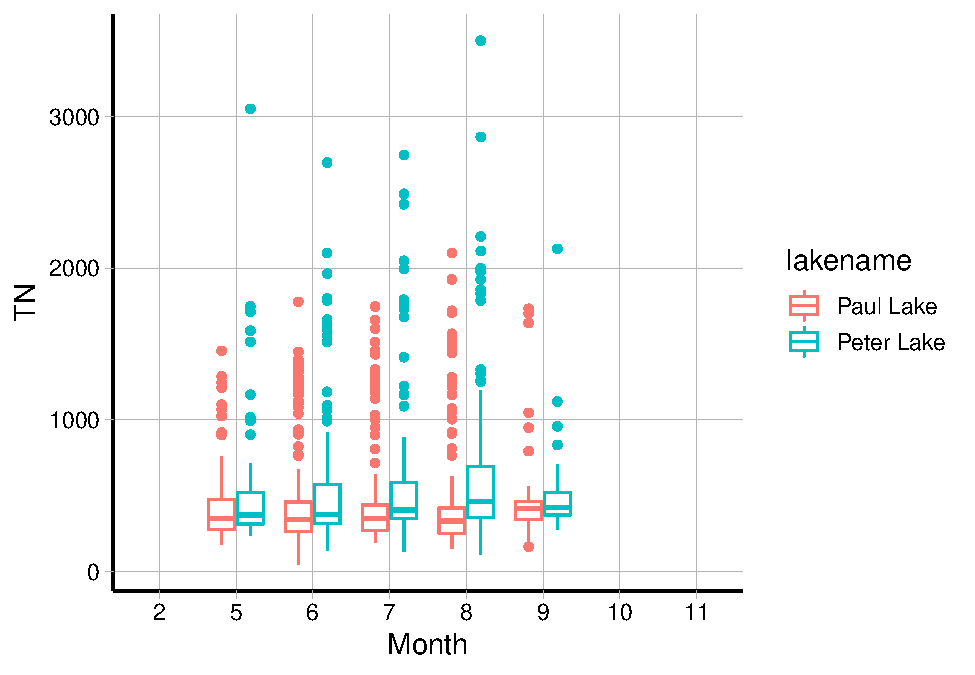
\includegraphics{A05_DataVisualization_files/figure-latex/unnamed-chunk-4-3.pdf}

\begin{Shaded}
\begin{Highlighting}[]
\CommentTok{\#fix this }
\NormalTok{PeterPaul.temp.TP.TN }\OtherTok{\textless{}{-}} \FunctionTok{plot\_grid}\NormalTok{(temp, TP, TN, }\FunctionTok{theme}\NormalTok{(}\AttributeTok{legend.position =} \StringTok{"bottom"}\NormalTok{), }\AttributeTok{nrow =}\DecValTok{3}\NormalTok{, }\AttributeTok{align =} \StringTok{\textquotesingle{}h\textquotesingle{}}\NormalTok{, }\AttributeTok{rel\_heights =} \FunctionTok{c}\NormalTok{(}\FloatTok{1.25}\NormalTok{, }\DecValTok{1}\NormalTok{))}
\end{Highlighting}
\end{Shaded}

\begin{verbatim}
## Warning: Removed 3566 rows containing non-finite values (stat_boxplot).
\end{verbatim}

\begin{verbatim}
## Warning: Removed 20729 rows containing non-finite values (stat_boxplot).
\end{verbatim}

\begin{verbatim}
## Warning: Removed 21583 rows containing non-finite values (stat_boxplot).
\end{verbatim}

\begin{verbatim}
## Warning in as_grob.default(plot): Cannot convert object of class themegg into a
## grob.
\end{verbatim}

\begin{verbatim}
## Warning: Graphs cannot be horizontally aligned unless the axis parameter is set.
## Placing graphs unaligned.
\end{verbatim}

\begin{Shaded}
\begin{Highlighting}[]
\FunctionTok{print}\NormalTok{(PeterPaul.temp.TP.TN)}
\end{Highlighting}
\end{Shaded}

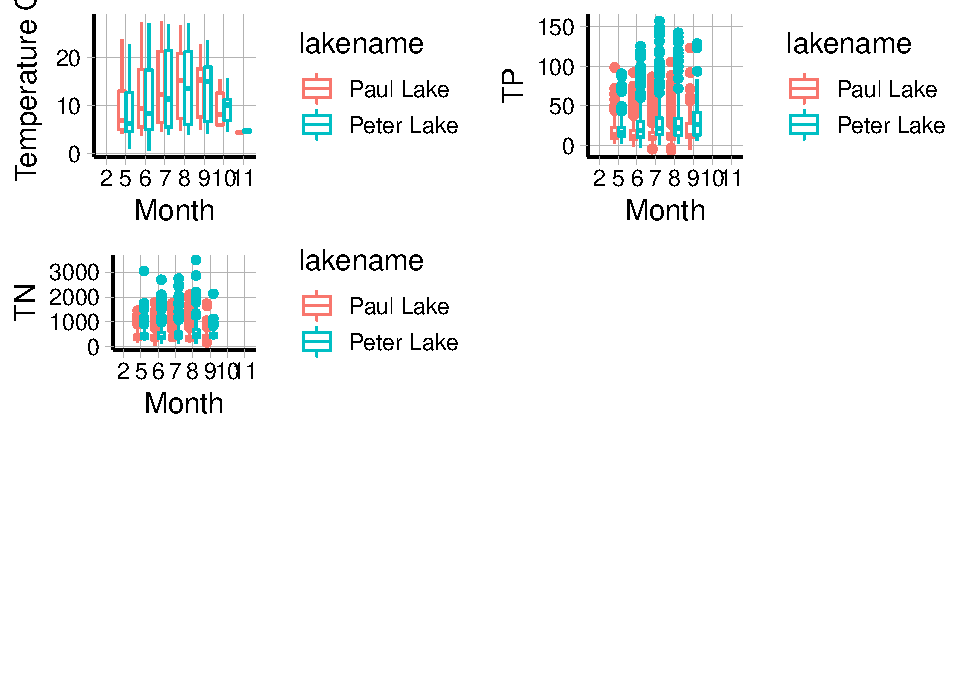
\includegraphics{A05_DataVisualization_files/figure-latex/unnamed-chunk-4-4.pdf}

Question: What do you observe about the variables of interest over
seasons and between lakes?

\begin{quote}
Answer: Over seasons and between lakes, the variables of interest appear
to follow similar trends.
\end{quote}

\begin{enumerate}
\def\labelenumi{\arabic{enumi}.}
\setcounter{enumi}{5}
\item
  {[}Niwot Ridge{]} Plot a subset of the litter dataset by displaying
  only the ``Needles'' functional group. Plot the dry mass of needle
  litter by date and separate by NLCD class with a color aesthetic. (no
  need to adjust the name of each land use)
\item
  {[}Niwot Ridge{]} Now, plot the same plot but with NLCD classes
  separated into three facets rather than separated by color.
\end{enumerate}

\begin{Shaded}
\begin{Highlighting}[]
\CommentTok{\#6}
\CommentTok{\#FIX THIS }
\NormalTok{needles }\OtherTok{\textless{}{-}} \FunctionTok{ggplot}\NormalTok{(}\FunctionTok{subset}\NormalTok{(litter, functionalGroup }\SpecialCharTok{\%in\%} \StringTok{"Needles"}\NormalTok{))}\SpecialCharTok{+}
  \FunctionTok{geom\_point}\NormalTok{(}\FunctionTok{aes}\NormalTok{(}\AttributeTok{x=}\NormalTok{collectDate, }\AttributeTok{y=}\NormalTok{dryMass,}\AttributeTok{color=}\NormalTok{nlcdClass)) }\SpecialCharTok{+}
\NormalTok{  mytheme}
\FunctionTok{print}\NormalTok{(needles)}
\end{Highlighting}
\end{Shaded}

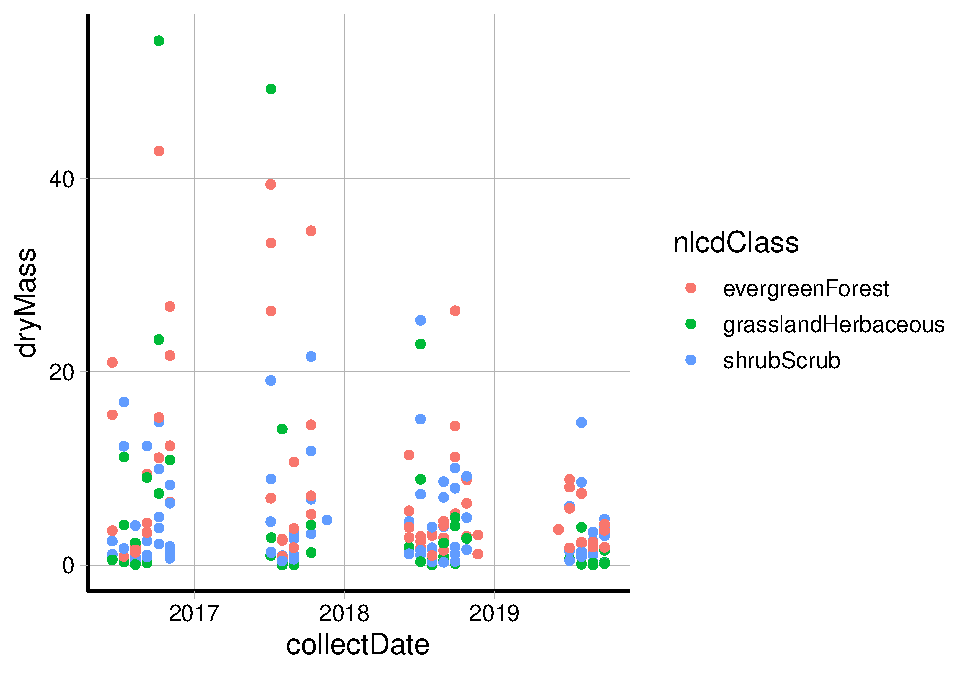
\includegraphics{A05_DataVisualization_files/figure-latex/unnamed-chunk-5-1.pdf}

\begin{Shaded}
\begin{Highlighting}[]
\CommentTok{\#7}
\NormalTok{needleSplit }\OtherTok{\textless{}{-}} \FunctionTok{ggplot}\NormalTok{(}\FunctionTok{subset}\NormalTok{(litter, functionalGroup }\SpecialCharTok{\%in\%} \StringTok{"Needles"}\NormalTok{))}\SpecialCharTok{+}
  \FunctionTok{geom\_point}\NormalTok{(}\FunctionTok{aes}\NormalTok{(}\AttributeTok{x=}\NormalTok{collectDate, }\AttributeTok{y=}\NormalTok{dryMass,}\AttributeTok{color=}\NormalTok{nlcdClass)) }\SpecialCharTok{+}
\NormalTok{  mytheme}
\FunctionTok{print}\NormalTok{(needles)}
\end{Highlighting}
\end{Shaded}

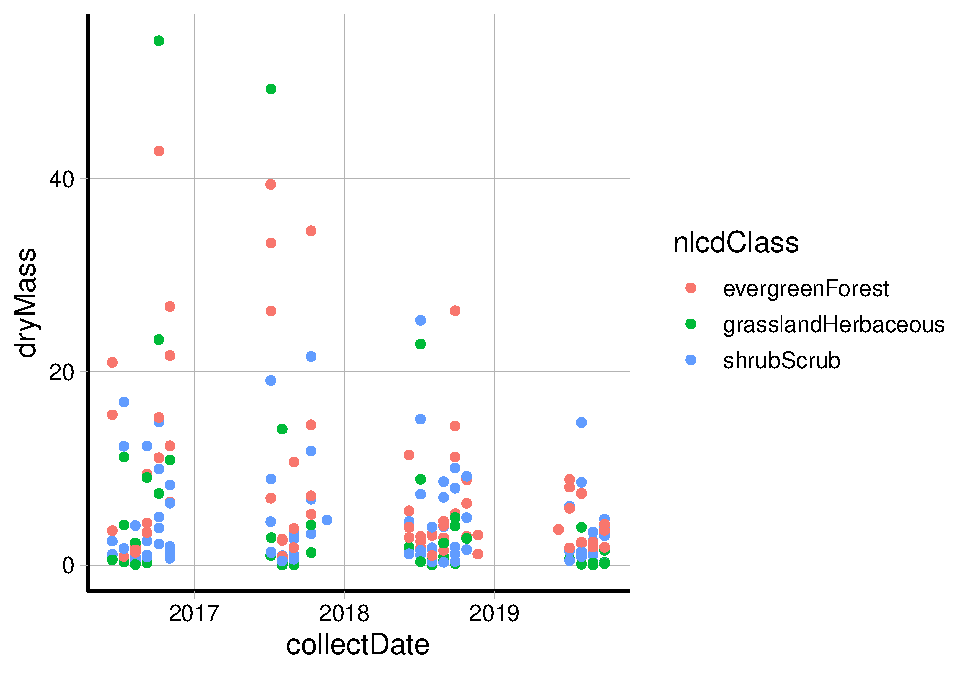
\includegraphics{A05_DataVisualization_files/figure-latex/unnamed-chunk-5-2.pdf}
Question: Which of these plots (6 vs.~7) do you think is more effective,
and why?

\begin{quote}
Answer:
\end{quote}

\end{document}
